\documentclass[a4paper]{article}
\usepackage[affil-it]{authblk}
\usepackage[english]{babel}
\usepackage[backend=bibtex,style=numeric]{biblatex}

\usepackage{geometry}
\geometry{margin=1.5cm, vmargin={0pt,1cm}}
\setlength{\topmargin}{-1cm}
\setlength{\paperheight}{29.7cm}
\setlength{\textheight}{25.3cm}

% useful packages.
\usepackage{amsfonts}
\usepackage{amsmath}
\usepackage{amssymb}
\usepackage{amsthm}     
\usepackage{enumerate} %enumerate environment
\usepackage{graphicx}
\usepackage{multicol}
\usepackage{fancyhdr}
\usepackage{layout}
\usepackage{ctex}      %中文环境
\usepackage{booktabs}  %三线表
\usepackage{verbatim}  %comment environment
\usepackage{float}     %强制表格图片位置
\usepackage{listings}  %insert code in latex
\usepackage{fontspec}  %font support
\usepackage{tikz}
\usepackage{makecell}
\usetikzlibrary{intersections}
\usepackage{arydshln}
\usepackage{mathptmx}
\usepackage{helvet}
\usepackage{courier}
\usepackage[colorlinks,linkcolor=blue]{hyperref}
\usepackage{xcolor}
\definecolor{mygreen}{rgb}{0,0.6,0}
\definecolor{lightgrey}{rgb}{0.95,0.95,0.95}
\definecolor{winered}{rgb}{0.5,0,0}
\definecolor{mymauve}{rgb}{0.58,0,0.82}
\lstset{
      backgroundcolor=\color{lightgrey},
      basicstyle             = \ttfamily,
      breakatwhitespace      = false,
      breaklines             = true,
      captionpos             = none,
      commentstyle           = \color{mygreen}\bfseries,
      extendedchars          = false,
      keepspaces             = true,
      keywordstyle           = \color{winered},         % keyword style
      language               = C++,                     % the language of code
      otherkeywords          = {string},
      numberstyle            = \tiny\color{mygray},
      rulecolor              = \color{black},
      showspaces             = false,
      showstringspaces       = false,
      showtabs               = false,
      stepnumber             = 1,
      stringstyle            = \color{mymauve},         % string literal style
      tabsize                = 2,
      title                  = \lstname,
      aboveskip              = 0pt,
      belowskip              = 0pt,
      columns                = flexible
}

% some common command
\newcommand{\dif}{\mathrm{d}}
\newcommand{\avg}[1]{\left\langle #1 \right\rangle}
\newcommand{\norm}[1]{\left\| #1 \right\|}
\newcommand{\difFrac}[2]{\frac{\dif #1}{\dif #2}}
\newcommand{\pdfFrac}[2]{\frac{\partial #1}{\partial #2}}
\newcommand{\OFL}{\mathrm{OFL}}
\newcommand{\UFL}{\mathrm{UFL}}
\newcommand{\fl}{\mathrm{fl}}
\newcommand{\op}{\odot}
\newcommand{\Eabs}{E_{\mathrm{abs}}}
\newcommand{\Erel}{E_{\mathrm{rel}}}
% \addbibresource{citation.bib}

\begin{document}
% =================================================
\title{Object-Oriented Programming report}

\author{Zhouyue Qian 3220104074
  \thanks{Electronic address: \texttt{3220104074@edu.zju.cn}}}
  
\affil{(Information and Computational Science Class 2201), Zhejiang University }


\date{Due time: \today}

\maketitle

\begin{abstract}
    This is an Object-Oriented Programming (OOP) project assignment. In this assignment, I accomplished the following tasks:
    \begin{enumerate}
      \item Implemented my own MyAllocate to replace \$stl::allocate\$.
      \item Utilized a memory pool to implement a simple memory pool.
    \end{enumerate}
    The project's code is located in the sr folder, which includes \$buffer.h\$, \$memory\_pool.h\$, \$allocate.h\$.
  \end{abstract}
  
  \section{Project Overview}

  This project implements a custom memory allocator \texttt{MyAllocate}, which is based on memory pool (\texttt{MemoryPool}) technology, aiming to optimize the performance of memory allocation and deallocation. \texttt{MyAllocate} is a template class that supports memory allocation and deallocation operations for any type. It implements the interface of the C++ Standard Library allocator, thus it can be seamlessly integrated with standard library containers such as \texttt{std::vector} and \texttt{std::list}.
  
  \section{Features}
  
  \begin{itemize}
      \item \textbf{Custom Memory Allocation}:
      \begin{itemize}
          \item Uses memory pool technology to optimize the performance of memory allocation and deallocation.
          \item Supports memory allocation for any type (via template parameter \texttt{T}).
      \end{itemize}
      \item \textbf{Standard Library Compatibility}:
      \begin{itemize}
          \item Implements the interface of the C++ Standard Library allocator, including \texttt{allocate}, \texttt{deallocate}, \texttt{construct}, and \texttt{destroy} methods.
          \item Supports seamless integration with \texttt{std::vector}, \texttt{std::list}, and other standard library containers.
      \end{itemize}
      \item \textbf{Memory Pool Management}:
      \begin{itemize}
          \item Uses the \texttt{MemoryPool} class to manage memory blocks, avoiding frequent calls to system-level \texttt{malloc} and \texttt{free}.
          \item The implementation of the memory pool ensures efficient memory allocation and deallocation.
      \end{itemize}
      \item \textbf{Type Safety}:
      \begin{itemize}
          \item Ensures type safety for memory allocation and deallocation through the template parameter \texttt{T}.
      \end{itemize}
      \item \textbf{Extensibility}:
      \begin{itemize}
          \item Supports allocator copying and rebinding operations, allowing allocators to be shared among different types.
      \end{itemize}
  \end{itemize}
  
  \section{Code Structure}
  
  \subsection{\texttt{allocator.h}}
  
  \texttt{allocator.h} is the core file of this project, containing the definition and implementation of the \texttt{MyAllocate} class. Here are the main parts:
  
  \begin{itemize}
      \item \textbf{Type Definitions}:
      \begin{itemize}
          \item \texttt{value\_type}, \texttt{pointer}, \texttt{const\_pointer}, \texttt{reference}, \texttt{const\_reference}, \texttt{size\_type}, and \texttt{difference\_type}.
      \end{itemize}
      \item \textbf{Constructors and Destructors}:
      \begin{itemize}
          \item Supports default construction, copy construction, and rebind construction.
          \item The destructor is responsible for releasing dynamically allocated resources.
      \end{itemize}
      \item \textbf{Memory Allocation and Deallocation}:
      \begin{itemize}
          \item \texttt{allocate(size\_type n, const void* hint = 0)}: Allocates memory for \texttt{n} objects.
          \item \texttt{deallocate(pointer p, size\_type n)}: Deallocates the memory pointed to by \texttt{p}.
      \end{itemize}
      \item \textbf{Object Construction and Destruction}:
      \begin{itemize}
          \item \texttt{construct(pointer ptr, const value\_type\& value)}: Constructs an object at the specified location.
          \item \texttt{destroy(pointer ptr)}: Destroys the object at the specified location.
      \end{itemize}
      \item \textbf{Address Operations}:
      \begin{itemize}
          \item \texttt{address(reference x)} and \texttt{address(reference x) const}: Returns the address of the object.
      \end{itemize}
      \item \textbf{Maximum Allocation Size}:
      \begin{itemize}
          \item \texttt{max\_size()}: Returns the maximum number of objects that the allocator can allocate.
      \end{itemize}
      \item \textbf{New Element Operations}:
      \begin{itemize}
          \item \texttt{newElement(const value\_type\& value)}: Allocates memory and constructs an object.
          \item \texttt{deleteElement(pointer p)}: Destroys the object and deallocates the memory.
      \end{itemize}
  \end{itemize}
  
  \subsection{\texttt{memory\_pool.h}}
  
  \texttt{memory\_pool.h} is the implementation file for the memory pool, responsible for managing the allocation and deallocation of memory blocks. Here are the main parts:
  
  \begin{itemize}
      \item \textbf{Memory Allocation}:
      \begin{itemize}
          \item \texttt{allocate(size\_t n)}: Allocates memory for \texttt{n} objects.
      \end{itemize}
      \item \textbf{Memory Deallocation}:
      \begin{itemize}
          \item \texttt{deallocate(T* p)}: Deallocates the memory pointed to by \texttt{p}.
      \end{itemize}
  \end{itemize}

  \section*{Results}
  The following results were obtained using the same random number seed.
  \begin{figure}[H]
    \centering
    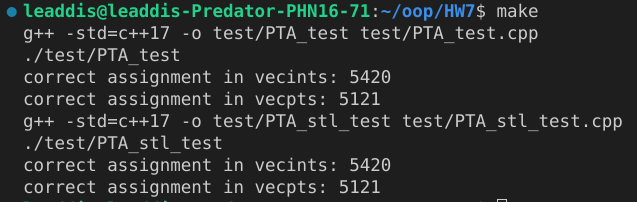
\includegraphics[width=0.8\textwidth]{result.png}
    \caption{Result Display 1}
  \end{figure}
  
  \begin{figure}[H]
    \centering
    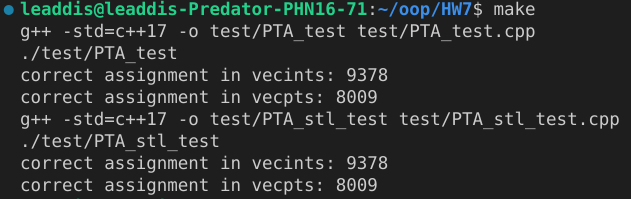
\includegraphics[width=0.8\textwidth]{result2.png}
    \caption{Result Display 2}
  \end{figure}

% ==============================================
% \section*{ \center{\normalsize {Acknowledgement}} }
% \printbibliography

\end{document}